% 2015-07-16 - Matthew A. Wolff - Thesis research presentation

\documentclass{beamer}

\mode<presentation> {
	% Themes and color schemes:
	\usetheme{default}
	\usecolortheme{rose}
}

% Need this on campus machine (but not at home)
%\usepackage{sansmathaccent}
%\pdfmapfile{+sansmathaccent.map}

\usepackage{graphicx} % Allows including images
\usepackage{booktabs} % Allows the use of \toprule, \midrule and \bottomrule in tables

%------------------------------------------------------------------------------
%	TITLE PAGE
%------------------------------------------------------------------------------

% The short title appears at the bottom of every slide, the full title is only on the title page
\title[Multilevel Summation Method]{Multilevel Summation Method} 

\author{Matthew A. Wolff} % Your name
\institute[Purdue University] % Your institution as it will appear on the bottom of every slide, may be shorthand to save space
{
	Purdue University \\ % Your institution for the title page
	\medskip
	\textit{wolff1@purdue.edu} % Your email address
}
\date{August 27, 2015} % Could also use \today, if desired

% Add slide numbers
\setbeamerfont{page number in head/foot}{size=\small}
\setbeamertemplate{footline}[frame number]

\begin{document}

\begin{frame}
	\titlepage % Print the title page as the first slide
\end{frame}

\begin{frame}
	\frametitle{Overview} % Table of contents slide, comment this block out to remove it
	\tableofcontents % Throughout your presentation, if you choose to use \section{} and \subsection{} commands, these will automatically be printed on this slide as an overview of your presentation
\end{frame}

\section{Timeline}

\frame{
	\frametitle{Timeline}

	\tiny{
		\begin{itemize}
			\item 7/20 - keep structure of error committed if basis function is omitted
			\item 7/20 - keep structure of error reduced by including basis function
			\item 7/21 - tried to determine "optimal" stencil size
			\item 7/25 - interpret finest grid as sum of interpolant and corrections
			\item 7/25 - interpolate on finest grid, push representation up grid hierarchy
			\item 7/25 - $\epsilon_\ell^{s_i} = \sum_{j=-p/2-\mu}^{p/2+\mu}{|\gamma(s_{i+j}) - \bar{\gamma}^{s_i}(s_{i+j})|}$ as error committed on grid $\ell$ by omitting basis function $s_i$
			\item 7/25 - built linear system defined by transferring coarse grid coefficients to fine grid coefficients
			\item 7/27 - linear time recurrence to get coarse grid coefficients from fine grid (inaccurate)
			\item 7/29 - worked on building linear system describing transfer from coarse to fine grids
			\item 7/31 - reworked how to represent linear system in such a way that it is nonsingular
			\item 8/3  - worked on quickly solving linear system
			\item 8/4  - worked on a (different) recurrence to solve linear system
			\item 8/5  - considered using Sherman-Morrison-Woodbury identity for linear system
			\item 8/6  - considered using Kenneth Miller recurrence for the inverse of a sum of matrices
			\item 8/7  - worked on runtime/storage complexity of multi-split, single-split(Skeel)
			\item 8/10 - worked on runtime/storage complexity of single-split(Wolff)
			\item 8/10 - proved that fine grid coefficients exist to exactly reproduce coarse grid values
			\item 8/17 - started analyzing interpolation error in 1D
			\item 8/22 - continued analyzing interpolation error in 1D
			\item 8/22 - algorithm for choosing parameters h, p, a,and k
			\item 8/23 - consider using various values of p at different levels
			\item 8/23 - determined what was being interpolated at each level, quasi-interpolation *should* simplify error analysis because interpolant is a polynomail of degree $p-1$
			\item 8/23 - computed initial total error estimate
			\item 8/24 - revised error analysis, view 1/r as "shifting" taylor expansion, quasi-interpolation is exact for first $p$ terms
			\item 8/24 - revised error analysis suggests that total error for $s \geq 1$ is $\frac{2}{s_i}$ where $s_i$ is grid point used in taylor expansion
			\item 8/24 - unfortunately, this analysis suggests that for even modest values of $\tau$, $10^8$ grid points are necessary on the coarsest grid
		\end{itemize}
	}
}

\small

\section{Main Ideas}

\frame{
	\frametitle{Main Ideas}

	\begin{itemize}
		\item Error committed by omitting basis function(s)
		\item Inefficient algorithm (complete)
		\item Efficient algorithm (incomplete)
		\item Error analysis in 1D
		\item *Parameter selection algorithm (h, p, a, and k)
		\item *Consider using different values of p on different grid levels
		\item **New interpretation of fine grid
	\end{itemize}

	\begin{itemize}
		\item *Unexplored, nothing ground-breaking
		\item **Proof of concept not yet finished
	\end{itemize}
}

\section{Basis Function Removal}

\frame{
	\frametitle{Basis Function Removal}
	
	Consider omitting a basis function, $s_i$, which will introduce errors at the $p/2+\mu$ neighboring grid points:
	\begin{center}
		\mbox{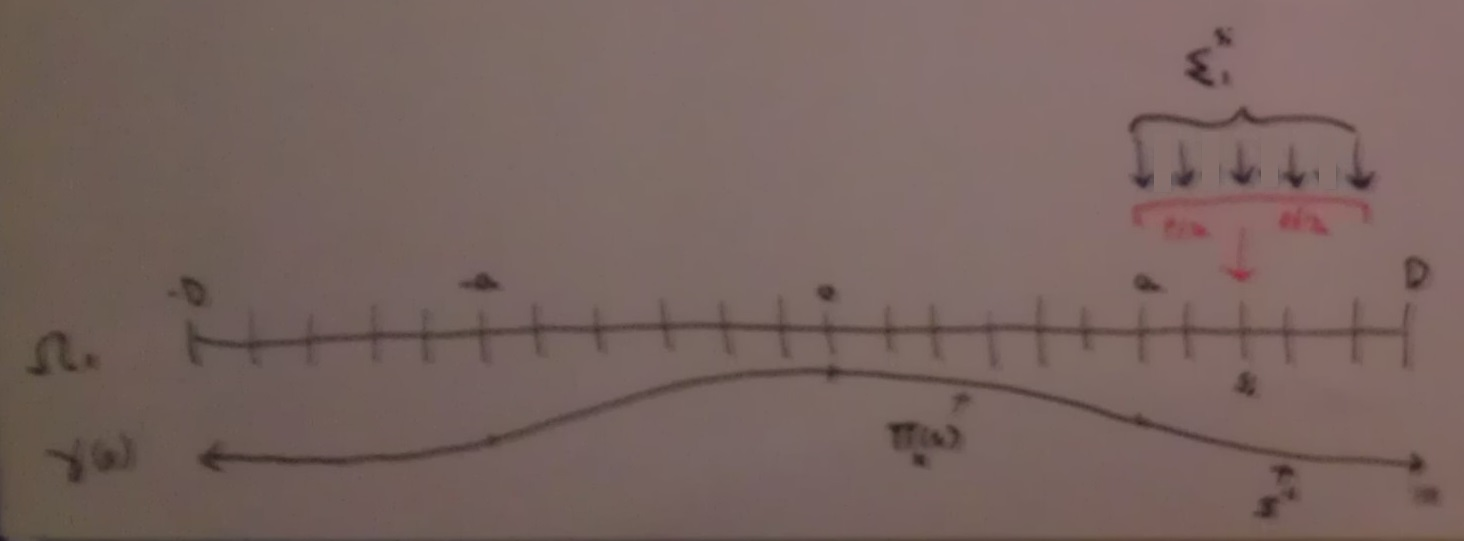
\includegraphics[width=0.9 \textwidth]{Figs/BFOmit.jpg}}
	\end{center}

	Represent the error committed on grid $\ell$ by omitting $s_i$ as:
	\[
		\epsilon_\ell^{s_i} = \sum_{j=-p/2-\mu}^{p/2+\mu}{|\gamma(s_{i+j}) - \bar{\gamma}^{s_i}(s_{i+j})|}
	\]
	where $\bar{\gamma}^{s_i}(s_k)$ is the interpolant evaluated at grid point $s_k$ without basis function $s_i$.
}

\frame{
	\frametitle{Basis Function Removal - 2}

	Note that:
	\begin{itemize}
		\item $\gamma(s)$ evaluation is either $O(1)$ or $O(k)$
		\item $\bar{\gamma}(s)$ evaluation could be $O(p)$ or $O(p\log{M})$
		\item $M$ is the number of grid points on the finest grid
		\item Total number of grid points on all levels is $O(M)$
		\item Assuming $\gamma$ and $\bar{\gamma}$ evaluation is negligible, computing error of each basis function removal is $O(M)$
	\end{itemize}
}

\section{Inefficient Algorithm}

%\frame{
%	\frametitle{Inefficient Algorithm}
%
%	\tiny{
%		\begin{itemize}
%			\item down-pass (to find all coefficients of basis functions)
%			\item up-pass (to remove any unnecessary basis functions)
%			\item 
%			\item 7/20 - keep structure of error committed if basis function is omitted
%			\item 7/20 - keep structure of error reduced by including basis function
%			\item 7/25 - $\epsilon_\ell^{s_i} = \sum_{j=-p/2-\mu}^{p/2+\mu}{|\gamma(s_{i+j}) - \bar{\gamma}^{s_i}(s_{i+j})|}$ as error committed on grid $\ell$ by omitting basis function $s_i$
%			%\item 8/7  - worked on runtime/storage complexity of multi-split, single-split(Skeel)
%		\end{itemize}
%	}
%}

\frame{
	\frametitle{Inefficient Algorithm}
		Down-Pass:
		\begin{itemize}
			\item Interpolate $\gamma(s)$ on coarsest grid, $\Omega^L$
			\item Compute interpolation error, $\Delta^{L-1}(s)$, on next finest grid, $\Omega^{L-1}$, at coarse-grid points and mid-points
			\item Set $\ell = L-1$
			\item Do:
			\begin{itemize}
				\item If $ \| \Delta^\ell(s) \| \leq \tau $, then exit loop
				\item Else, interpolate $\Delta^\ell(s)$ on $\Omega^\ell$
				\item Compute updated interpolation error, $\Delta^{\ell-1}$, on next finest grid, $\Omega^{\ell-1}$, at points and midpoints of $\Omega^\ell$
				\item Set $\ell = \ell - 1$
				\item Repeat
			\end{itemize}
		\end{itemize}
}

\frame{
	\frametitle{Inefficient Algorithm}
		Up-Pass:
		\begin{itemize}
			\item $\ell = 1$
			\item For $\ell < L$
			\begin{itemize}
				\item For each $s_i$, from "outside" towards "inside"
				\begin{itemize}
					\item if $\epsilon_{\ell}^{s_i} \leq \tau$, check next $s_i$
					\item else, exit loop
				\end{itemize}
			\end{itemize}
			\item $\ell = \ell + 1$
	\end{itemize}
	Note: $\tau$ is some specified tolerance
}

%\frame{
%	\frametitle{How to compute stencils?}
%	Define the following:
%	\begin{itemize}
%		\item $f(x)$ is objective function
%		\item $\bar{f}^\ell(x)$ is interpolant of $f(x)$ using grids $\Omega^\ell$ through $\Omega^L$
%		\item $\Delta^\ell(x)$ is interpolation error of $\bar{f}^{\ell+1}$
%		\begin{itemize}
%			\item $\Delta^\ell(x) = f(x) - \bar{f}^{\ell+1}$
%		\end{itemize}
%		\item $\hat{\Delta}^\ell(x)$ is anti-blurred $\Delta^\ell(x)$ (i.e. stencil of coefficients)
%		\begin{itemize}
%			\item $\hat{\Delta}^\ell(x) = \mathcal{A} \Delta^\ell(x)$
%		\end{itemize}
%		\item $\bar{\Delta}^\ell(x)$ is interpolant of $\Delta^\ell(x)$
%		\begin{itemize}
%			\item $\bar{\Delta}^\ell(x) = \mathcal{B} \mathcal{A} \Delta^\ell(x)$
%		\end{itemize}
%	\end{itemize}
%	
%	Then, using the coarsest $\ell$ grids, the interpolant is given by
%	\[ \bar{f}^\ell(x) = \bar{f}^L(x) + \bar{\Delta}^{L-1}(x) + \dots + \bar{\Delta}^{\ell+1}(x) + \bar{\Delta}^\ell(x) = \bar{f}^{\ell+1} + \bar{\Delta}^\ell(x) \]
%}

\section{Efficient Algorithm}

%\frame{
%	\frametitle{Efficient Algorithm}
%
%	\tiny{
%		\begin{itemize}
%			\item down-pass with predetermined stencil sizes (to find all necessary basis functions)
%			\item 
%			\item 7/21 - tried to determine "optimal" stencil size
%			\item 7/25 - $\epsilon_\ell^{s_i} = \sum_{j=-p/2-\mu}^{p/2+\mu}{|\gamma(s_{i+j}) - \bar{\gamma}^{s_i}(s_{i+j})|}$ as error committed on grid $\ell$ by omitting basis function $s_i$
%			%\item 8/7  - worked on runtime/storage complexity of multi-split, single-split(Skeel)
%			\item 8/17 - started analyzing interpolation error in 1D
%			\item 8/22 - continued analyzing interpolation error in 1D
%			\item 8/22 - algorithm for choosing parameters h, p, a,and k
%			\item 8/23 - consider using various values of p at different levels
%			\item 8/23 - determined what was being interpolated at each level, quasi-interpolation *should* simplify error analysis because interpolant is a polynomail of degree $p-1$
%			\item 8/23 - computed initial total error estimate
%			\item 8/24 - revised error analysis, view 1/r as "shifting" taylor expansion, quasi-interpolation is exact for first $p$ terms
%			\item 8/24 - revised error analysis suggests that total error for $s \geq 1$ is $\frac{2}{s_i}$ where $s_i$ is grid point used in taylor expansion
%			\item 8/24 - unfortunately, this analysis suggests that for even modest values of $\tau$, $10^8$ grid points are necessary on the coarsest grid
%		\end{itemize}
%	}
%}

\frame{
	\frametitle{Efficient Algorithm}
		Down-Pass:
		\begin{itemize}
			\item Interpolate $\gamma(s)$ on coarsest grid, $\Omega^L$
			\item Compute interpolation error, $\Delta^{L-1}(s)$, on next finest grid, $\Omega^{L-1}$, at coarse-grid points and mid-points
			\item Compute $\epsilon_{L}^{s_i}$ for each basis function $s_i$ from the \textbf{inside-out}, stopping if $\epsilon_{L}^{s_i} \leq \tau$
			\item Set $\ell = L-1$
			\item Do:
			\begin{itemize}
				\item If $ \| \Delta^\ell(s) \| \leq \tau $, then exit loop
				\item Else, interpolate $\Delta^\ell(s)$ on $\Omega^\ell$
				\item Compute updated interpolation error, $\Delta^{\ell-1}$, on next finest grid, $\Omega^{\ell-1}$, at points and midpoints of $\Omega^\ell$
				\item Compute $\epsilon_{\ell}^{s_i}$ for each basis function $s_i$ from the \textbf{inside-out}, stopping if $\epsilon_{\ell}^{s_i} \leq \tau$
				\item Set $\ell = \ell - 1$
				\item Repeat
			\end{itemize}
		\end{itemize}
		Note: Updating interpolation error and examining basis function omission could probably happen simultaneously
}

\section{Error Analysis}

\frame{
	\frametitle{Error Analysis}
	From paper, 1D B-Spline interpolation yields error:
	\[
		\left( \frac{Ch}{2} \right)^p ||\gamma(\zeta)^{(p)}||_{\infty}
	\]
	where $h$ is grid spacing, $C$ is a value based on $p$, and $\gamma(\zeta)^{(p)}$ is the $p^{\text{th}}$ derivative of $\gamma(s)$ evaluated at some point $\zeta$.
}

\frame{
	\frametitle{Error Analysis - 2}
	Thus, for
	\[
		\gamma(s) = 
		\begin{cases}
			c_0 + c_1 s^2 + \dots + c_k s^{2k}, & 0 \leq s < 1 \\
			\frac{1}{s}, & s \geq 1
		\end{cases}
	\]

	we have:
	\[
		\gamma(s)^{(p)} = 
		\begin{cases}
			(p!) c_{p/2} + \frac{(p+2)!}{2!} c_{p/2+1} s^2 + \dots + \frac{(2k)!}{(2k-p)!} c_k s^{2k-p}, & 0 \leq s < 1 \\
			\frac{(-1)^p (p!)}{s^{p+1}}, & s \geq 1
		\end{cases}
	\]

	Note:
	\begin{enumerate}
		\item If $k = p/2 - 1$, then quasi-interpolation should be exact for polynomail on $0 \leq s < 1$
		\begin{itemize}
			\item Otherwise, we could use optimization technique to find $||\gamma^{(p)}(\zeta)||\infty$
		\end{itemize}
		\item For $s \geq 1$, maximum happens at $s=1$ and rapidly drops off
	\end{enumerate}
}

\frame{
	\frametitle{Error Analysis - 3}

	\tiny{*My logic may be flawed here.}

	Furthermore, for $s \geq 1$:
	\begin{itemize}
		\item B-Spline interpolant, $\bar{\gamma}(s)$, when evaluated at $s$ is the sum of degree $p-1$ polynomials.
		\item $\gamma(s) = \gamma(s_i) + \frac{\gamma^{(1)}(s_i)}{1!}(s-s_i) + \frac{\gamma^{(2)}(s_i)}{2!}(s-s_i)^2 + \dots + \frac{\gamma^{(n)}(s_i)}{n!}(s-s_i)^n + \dots$
		\item $\gamma(s) - \bar{\gamma}(s) = \frac{\gamma^{(p)}(s_i)}{p!}(s-s_i)^p + \frac{\gamma^{(p+1)}(s_i)}{(p+1)!}(s-s_i)^{p+1} + \dots $
		\item $\Rightarrow \gamma(s) - \bar{\gamma}(s) = \frac{(-1)^p}{(s_i)^{p+1}}(s-s_i)^p  + \frac{(-1)^{p+1}}{(s_i)^{p+2}}(s-s_i)^{p+1} + \dots $
		\item Let $s = s_i + 1$, then $\gamma(s) - \bar{\gamma}(s) = \frac{(-1)^p}{(s_i)^{p+1}}  + \frac{(-1)^{p+1}}{(s_i)^{p+2}} + \dots $ 
		\item $\Rightarrow \gamma(s) - \bar{\gamma}(s) \rightarrow 0 \text{ as } s_i \rightarrow \infty$
		\item Taking $\tau$ into account, should yield a basis function $s_i$ such that the approximation is within the tolerance
	\end{itemize}
}

\frame{
	\frametitle{The End!}
	\begin{center}
		Thank you!
	\end{center}
}

%\section{A different interpretation}
%
%%\frame
%%{
%%	\frametitle{A different interpretation}
%%
%%	\tiny{
%%		\begin{itemize}
%%			\item interpolate on fine grid (to get all basis function coefficients)
%%			\item compute coefficients for "next-coarsest" grid until coefficients on coarsest grid (to transfer coefficients and transform representation)
%%			\item no intermediate direct computations, just anterpolation, direct coarse part, interpolation (approx 3x faster evals)
%%			\item 
%%			\item 7/25 - interpret finest grid as sum of interpolant and corrections
%%			\item 7/25 - interpolate on finest grid, push representation up grid hierarchy
%%			\item 7/25 - built linear system defined by transferring coarse grid coefficients to fine grid coefficients
%%			\item 7/27 - linear time recurrence to get coarse grid coefficients from fine grid (inaccurate)
%%			\item 7/29 - worked on building linear system describing transfer from coarse to fine grids
%%			\item 7/31 - reworked how to represent linear system in such a way that it is nonsingular
%%			\item 8/3  - worked on quickly solving linear system
%%			\item 8/4  - worked on a (different) recurrence to solve linear system
%%			\item 8/5  - considered using Sherman-Morrison-Woodbury identity for linear system
%%			\item 8/6  - considered using Kenneth Miller recurrence for the inverse of a sum of matrices
%%			\item 8/10 - proved that fine grid coefficients exist to exactly reproduce coarse grid values
%%			%\item 8/10 - worked on runtime/storage complexity of single-split(Wolff)
%%		\end{itemize}
%%	}
%%}
%
%\frame
%{
%	\frametitle{A different interpretation}
%}

%%*-*-*-*-*-*-*-*-*-*-*-*-*-*-*-*-*-*-*-*-*-*-*-*-*-*-*-*-*-*-*-*-*-*-*-
%%* MSM with Single Splitting
%%*-*-*-*-*-*-*-*-*-*-*-*-*-*-*-*-*-*-*-*-*-*-*-*-*-*-*-*-*-*-*-*-*-*-*-
%\section{Single Splitting}
%
%\frame{
%	\frametitle{What?, Why?, When?, Where?, How?}
%	\begin{itemize}
%		\item What: Split the kernel once
%		\item Why: The term which is interpolated has infinite extent
%		\item When: Explicitly when forming the algorithm
%		\item Where: The long-range part of the kernel
%		\item How: This will be the focus of today's presentation
%	\end{itemize}
%}
%
%\frame{
%	\frametitle{What?}
%
%	Split the computational kernel once:
%	\begin{itemize}
%		\item $k(\textbf{r},\textbf{r}') = \frac{1}{\| \textbf{r}' - \textbf{r} \|}$
%		\item $k(\textbf{r},\textbf{r}') = k_0(\textbf{r},\textbf{r}') + k_1(\textbf{r},\textbf{r}')$
%		\begin{itemize}
%			\item "Short-range" component, $k_0$, is computed exactly via geometric hashing
%			\item "Long-range" component, $k_1$, is interpolated on a hierarchy of grids
%		\end{itemize}
%	\end{itemize}
%}
%
%\frame{
%	\frametitle{Why?}
%
%	In general, interpolation using B-Splines can be shown to have the form:
%	\[ \bar{f}(x) = \sum_n{f_n^\ell\phi_n^\ell(x)} \]
%	where
%	\begin{itemize}
%		\item $\bar{f}(x)$ is the interpolant
%		\item $f_m^\ell = \sum_n{\omega_{m-n}f(nh_\ell)}$
%		\item $f(x)$ is continuous, bounded objective function
%		\item $\phi_n^\ell(x) = \Phi(x/h_\ell - n)$
%	\end{itemize}
%
%	\vspace{0.2in}
%
%	So, single-split because
%	\begin{itemize}
%		\item B-Spline interpolant of a function with compact support is not compact
%%		\item FIXME: pic of exaggerated function and interpolant
%		\item Long-range component does not have compact support
%	\end{itemize}
%}
%
%\frame{
%	\frametitle{How?}
%
%	Algorithmic overview:
%	\begin{itemize}
%		\item Interpolate function, $f(x)$, on coarsest grid, $\Omega^L$
%		\item Compute interpolation error, $\Delta^{L-1}(x)$, on next finest grid, $\Omega^{L-1}$, at coarse-grid points and mid-points
%		\item Do:
%		\begin{itemize}
%			\item If $ \| \Delta^\ell(x) \| \leq \tau $, then exit loop
%			\item Else, interpolate $\Delta^\ell(x)$ on $\Omega^\ell$
%			\item Compute updated interpolation error, $\Delta^{\ell-1}$, on next finest grid, $\Omega^{\ell-1}$, at points and midpoints of $\Omega^\ell$
%			\item Set $\ell = \ell - 1$
%			\item Repeat
%		\end{itemize}
%	\end{itemize}
%}
%
%\frame{
%	\frametitle{How? - Example}	% f(x)
%	\begin{center}
%		\mbox{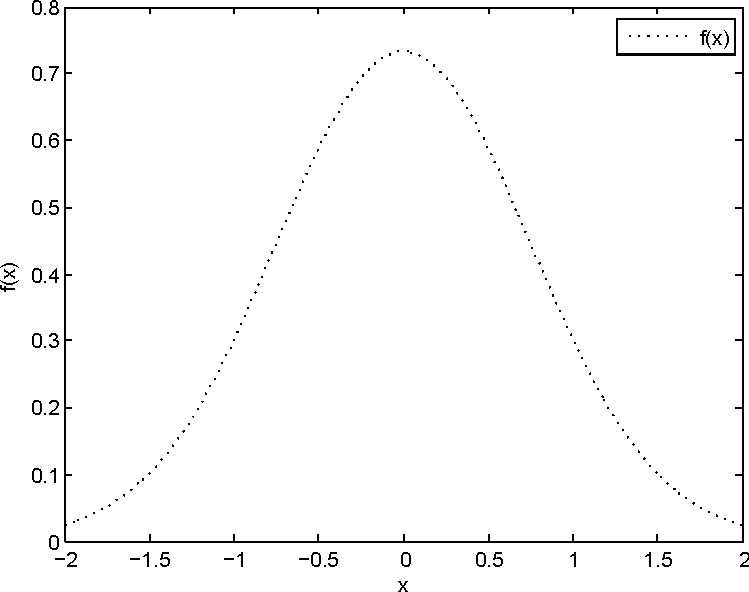
\includegraphics[width=0.9 \textwidth]{Figs/Refine1.pdf}}
%	\end{center}
%	\[ \text{ }  \]
%}
%
%\frame{
%	\frametitle{How? - Example}	% f(x), f_1(x)
%	\begin{center}
%		\mbox{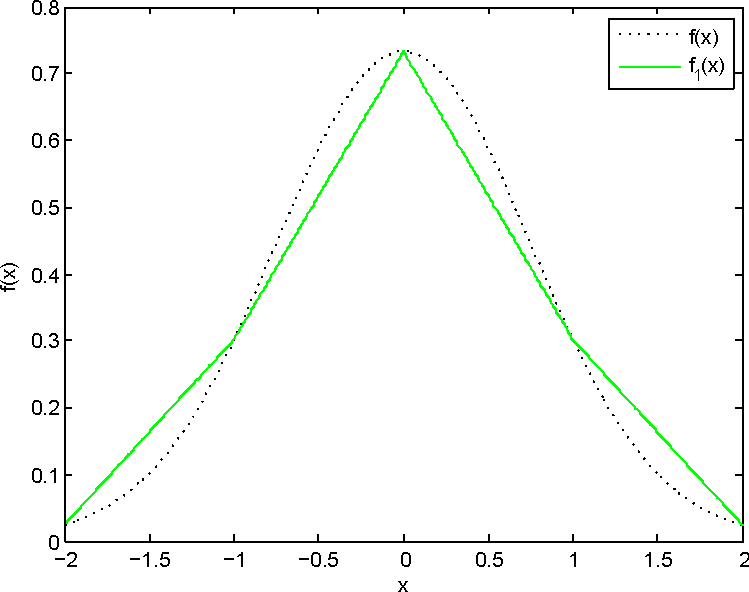
\includegraphics[width=0.9 \textwidth]{Figs/Refine2.pdf}}
%	\end{center}
%	\[ f(x) \approx \textcolor{green}{f_1(x)}  \]
%}
%
%\frame{
%	\frametitle{How? - Example}	% f(x), f_1(x), f_2(x)
%	\begin{center}
%		\mbox{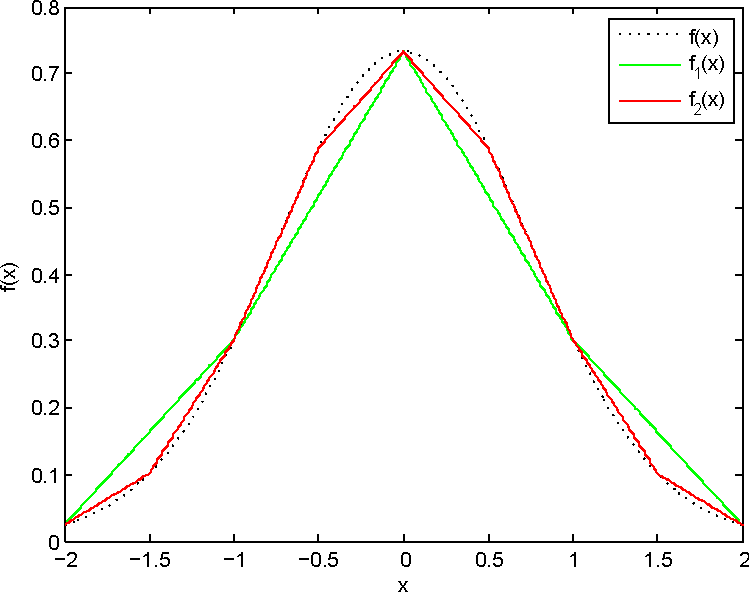
\includegraphics[width=0.9 \textwidth]{Figs/Refine3.pdf}}
%	\end{center}
%	\[ f(x) \approx \textcolor{red}{f_2(x)} = \textcolor{green}{f_1(x)} + \Delta^2(x) \]
%}
%
%\frame{
%	\frametitle{How? - Example}	% f(x), f_1(x), f_2(x), f_3(x)
%	\begin{center}
%		\mbox{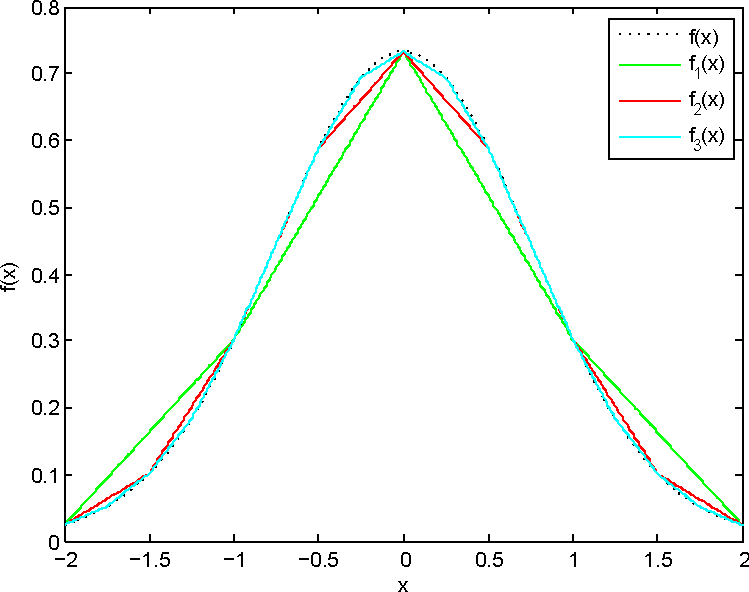
\includegraphics[width=0.9 \textwidth]{Figs/Refine4.pdf}}
%	\end{center}
%	\[ f(x) \approx \textcolor{cyan}{f_3(x)} = \textcolor{green}{f_1(x)} + \textcolor{red}{\Delta^2(x)} + \Delta^3(x) = \textcolor{red}{f_2(x)} + \Delta^3(x)  \]
%}
%
%\frame{
%	\frametitle{How? (Continued)}
%	Currently, two main questions:
%	\begin{enumerate}
%		\item How to compute stencils?
%		\item How to remove basis functions?
%	\end{enumerate}
%}
%
%\subsection{How to compute stencils?}
%
%\frame{
%	\frametitle{How to compute stencils?}
%	Define the following:
%	\begin{itemize}
%		\item $f(x)$ is objective function
%		\item $\bar{f}^\ell(x)$ is interpolant of $f(x)$ using grids $\Omega^\ell$ through $\Omega^L$
%		\item $\Delta^\ell(x)$ is interpolation error of $\bar{f}^{\ell+1}$
%		\begin{itemize}
%			\item $\Delta^\ell(x) = f(x) - \bar{f}^{\ell+1}$
%		\end{itemize}
%		\item $\hat{\Delta}^\ell(x)$ is anti-blurred $\Delta^\ell(x)$ (i.e. stencil of coefficients)
%		\begin{itemize}
%			\item $\hat{\Delta}^\ell(x) = \mathcal{A} \Delta^\ell(x)$
%		\end{itemize}
%		\item $\bar{\Delta}^\ell(x)$ is interpolant of $\Delta^\ell(x)$
%		\begin{itemize}
%			\item $\bar{\Delta}^\ell(x) = \mathcal{B} \mathcal{A} \Delta^\ell(x)$
%		\end{itemize}
%	\end{itemize}
%	
%	Then, using the coarsest $\ell$ grids, the interpolant is given by
%	\[ \bar{f}^\ell(x) = \bar{f}^L(x) + \bar{\Delta}^{L-1}(x) + \dots + \bar{\Delta}^{\ell+1}(x) + \bar{\Delta}^\ell(x) = \bar{f}^{\ell+1} + \bar{\Delta}^\ell(x) \]
%}
%
%\subsection{How to remove basis functions?}
%
%\frame{
%	\frametitle{How to remove basis functions?}
%
%%	\begin{itemize}
%%		\item Which basis function(s) \it{can} be removed?
%%	\end{itemize}
%	Rearrange terms in interpolant as follows:
%	\[ \bar{f}^\ell(x) = \bar{f}^{\ell+} + \bar{f}^{\ell-}  \]
%	where
%	\begin{itemize}
%		\item $\bar{f}^{\ell+}$ are terms with \textbf{required} basis functions
%		\item $\bar{f}^{\ell-}$ are terms with \textbf{unnecessary} basis functions
%	\end{itemize}
%
%	Now, we have:
%	\begin{align}
%		f(x) &= \bar{f}^\ell(x) + \Delta^{\ell-1} \\
%		&= \bar{f}^{\ell+} + \bar{f}^{\ell-} + \Delta^{\ell-1}
%	\end{align}
%	
%	and we want to stop at level $\ell$ when
%	\begin{align}
%		\| f(x) - \bar{f}^{\ell+}(x) \| &\leq \tau \\
%		\| \bar{f}^{\ell-} + \Delta^{\ell-1} \| &\leq \tau
%	\end{align}
%}
%
%%\section{Roadmap to completion}
%%
%%\frame{
%%	\frametitle{Roadmap to Completion}
%%	Overview:
%%	\begin{itemize}
%%		\item Single-split MSM
%%		\begin{itemize}
%%			\item Update pre-processing to build stencil for each grid level
%%			\item Force evaluation code largely unaffected
%%			\begin{itemize}
%%				\item Update direct calculation routine to use stencil-specific radius
%%			\end{itemize}
%%			\item Compare accuracy to multi-split version
%%		\end{itemize}
%%	\end{itemize}
%%}
%
%\section{Conclusion}
%
%\frame{
%	\frametitle{Conclusion}
%
%	Need to
%	\begin{itemize}
%		\item Find $\bar{f}^{\ell-}$ and round those coefficients to zero
%		\item Find optimal way to do this for minimal computational complexity
%	\end{itemize}
%}
%
%%\frame{
%%	\frametitle{The end}
%%	\begin{center}
%%		Thank you!
%%	\end{center}
%%}
%
%%\frame{
%%	\frametitle{Bibliography}
%%	\begin{itemize}
%%		\item \tiny{A. Brandt and A. Lubrecht, \textit{Multilevel Matrix Multiplication and Fast Solution of Integral Equations}, J. Comp. Phys., 90 (1990), pp. 348-370.}
%%		\item \tiny{A. Brandt and C. Venner, \textit{Multilevel Evaluation of Integral Transforms with Asympotically Smooth Kernels}, SIAM J. Sci. Comput., Vol. 19, No. 2 (1998), pp. 468 - 492.}
%%		\item \tiny{D. Hardy. \textit{Multilevel Summation for the Fast Evaluation of Forces for the Simulation of Biomolecules}. PhD thesis, Univ. of Illinois at Urbana-Champaign, 2006.}
%%		\item \tiny{M. Griebel, S. Knapek, and G. Zumbusch, \textit{Numerical simulation in molecular dynamics}, Springer (2007).}
%%		\item \tiny{D. Hardy, J. Stone, and K. Schulten, \textit{Multilevel summation of electrostatic potentials using graphics processing units}, Parallel Computing, 35 (2009), pp. 164 - 177.}
%%		\item \tiny{S. Moore and P. Crozier, \textit{Extension and evaluation of the multilevel summation method for fast long-range electrostatics calculations}, J. Chem. Phys., 140 (2014), pp. 234112-1 - 234112-12.}
%%		\item \tiny{D. Tameling, P. Springer, P. Bientinesi, and A. Ismail, \textit{Multilevel summation for dispersion: A linear time algorithm for $r^{-6}$ potentials}, J. Chem. Phys., 140 (2014), pp. 024105-1 - 024105-12.}
%%		\item \tiny{D. Hardy, M. Wolff, J. Xia, K. Schulten, R. Skeel, \textit{Multilevel Summation Using B-Spline Interpolation}, In preparation (2015).}
%%	\end{itemize}
%%}

\end{document}